% Chapter 5

\chapter{Project Outcome} % Chapter title

\label{ch:outcome} 
% For referencing the chapter elsewhere, use \autoref{ch:outcome} 

%----------------------------------------------------------------------------------------

The project ended up with a web-based project management system.
The system consists of basic managing features which cover most common scenarios in PMT.
Besides that, the system also follows a set of MLS policies described in \autoref{ch:background:bell}.
This chapter includes an installation guide to setup the project from fresh; 
the system's user guide which describes its features and their usage demonstrations.
And at the end, I will discuss about my learning from the project's developing progress.

%----------------------------------------------------------------------------------------

\section{Installation Guide}
\label{ch:result:installation_guide}

\autoref{ch:implementation:technical_information} listed the technical requirements for this project.
In this guide, we will learn about the project's setup from scratch, step by step.

Assume that you already have a machine running CentOS 7 with these packages have already been installed: \emph{git, postgresql, nodejs with npm}.
I am using \emph{Digital Ocean} as VPS provider.
I create a \emph{Digital Ocean's droplet} with this specification: \emph{512MB Ram 20GB SSD Disk CentOS 7.1 x64}.
A postgresql database should be created and named as \emph{hotpot} whose owner is \emph{hotpot} and the password at your own choice.

First of all we need to clone the project's source code from GitHub using the command.
\begin{lstlisting}[breaklines=false,frame=lt]
$ git clone git@github.com:khangpn/hotpot.git
\end{lstlisting}

Next, we need to install all the project's dependencies by going into the project's root directory and execute \emph{npm} install command
\begin{lstlisting}[breaklines=false,frame=lt]
$/hotpot/ npm install
\end{lstlisting}
This command may take a while to install all required packages.

After checking the database accessibility, we need to configure its connection in \emph{config\/database.js}. 
Open that file by your favorite text editor, my choice is \emph{vim}. 
\begin{lstlisting}[breaklines=false,frame=lt]
$/hotpot/ vim config/database.js
\end{lstlisting}

Below is an example of the database configuration, if you named the database, its user and password are \emph{hotpot} and the database is running on local machine, then your configuration file should be similar to this.
\begin{lstlisting}[breaklines=false,frame=lt]
var settings = {                                                                                                                                                     
  development: { 
    database : "hotpot",
    username : "hotpot",
    password : "hotpot",
    options  : { 
      dialect : "postgresql",
      host     : "127.0.0.1"   
    }
  },
  production: { 
    database : "hotpot",
    username : "hotpot",
    password : "hotpot",
    options  : { 
      dialect : "postgresql",  
      host     : "127.0.0.1"   
    }
  }
};
  
module.exports = settings;
\end{lstlisting}

Next, lets open file \emph{setup} and change its \emph{NODE\_ENV} to \emph{development} or \emph{production} depending on your purpose.
\emph{Development} environemnt will print out the system's logs on our server and return errors' full stack trace to client, while  \emph{production} will omit it.
\begin{lstlisting}[breaklines=false,frame=lt]
// file hotpot/setup
NODE_ENV=development DEBUG=hotpot node bin/db-integration.js
\end{lstlisting}

Also edit file \emph{start} to change its \emph{NODE\_ENV}
\begin{lstlisting}[breaklines=false,frame=lt]
// file hotpot/start
NODE_ENV=development DEBUG=hotpot npm start
\end{lstlisting}
We can also add \emph{PORT} variable to the script to specify the project's running port. By default, it runs on port \emph{3000}
\begin{lstlisting}[breaklines=false,frame=lt]
// file hotpot/start
NODE_ENV=development PORT=4000 DEBUG=hotpot npm start
\end{lstlisting}

Next, we have to initialize the project's database schema using the \emph{setup} script.
\begin{lstlisting}[breaklines=false,frame=lt]
$/hotpot/ ./setup
\end{lstlisting}
This setup may take a while. And finally we can start the project using the \emph{start} script.
\begin{lstlisting}[breaklines=false,frame=lt]
$/hotpot/ ./start
\end{lstlisting}

%----------------------------------------------------------------------------------------

\section{User Guide}
\label{ch:result:user_guide}

As the demonstration for this project, I have deployed \myProject at the address \href{http://178.62.253.47:3000/}{http://178.62.253.47:3000/}.
In this section, we are going through demonstrations of the project's features \ie test cases of the project's behaviours.

% Miscellaneous guide ----------------------------
\subsection{Miscellaneous}
\label{ch:result:user_guide:miscellaneous}
\autoref{fig:user_guide:homepage}, \autoref{fig:user_guide:user_interface}, \autoref{fig:user_guide:admin_interface},\autoref{fig:user_guide:profile}, and \autoref{fig:user_guide:not_permitted} are some general interfaces which are visible across the guide.

\begin{figure}[bth]                                                                                                                                                  \myfloatalign
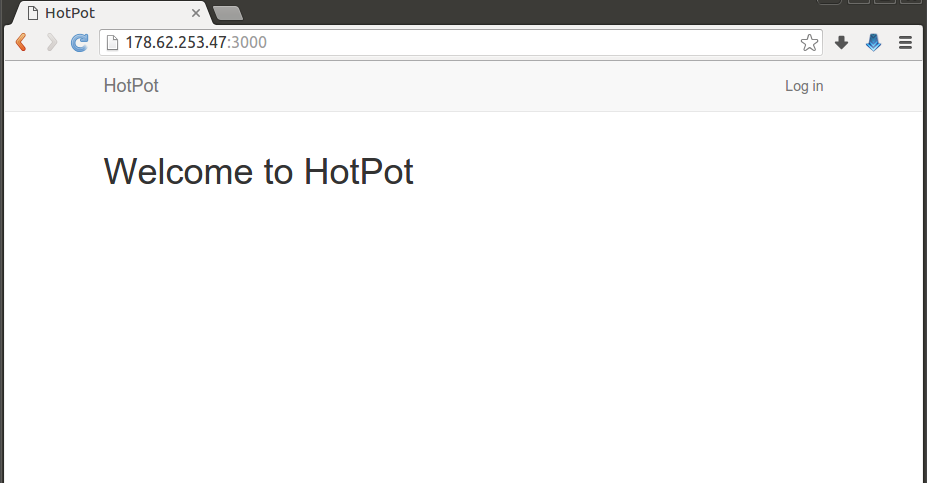
\includegraphics[width=1.0\linewidth]{gfx/chapter_5/general/homepage}
\caption[HotPot homepage]{HotPot homepage}
\label{fig:user_guide:homepage}
\end{figure}

\begin{figure}[bth]                                                                                                                                                  \myfloatalign
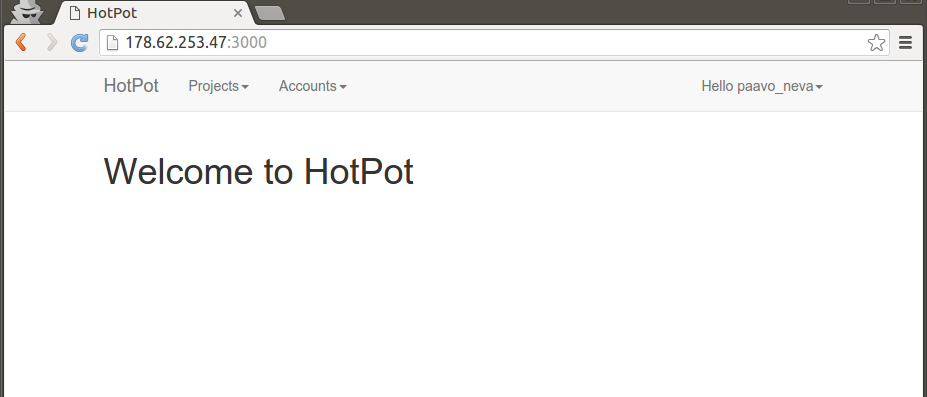
\includegraphics[width=1.0\linewidth]{gfx/chapter_5/general/user_interface}
\caption[HotPot user interface]{HotPot user interface}
\label{fig:user_guide:user_interface}
\end{figure}

\begin{figure}[bth]                                                                                                                                                  \myfloatalign
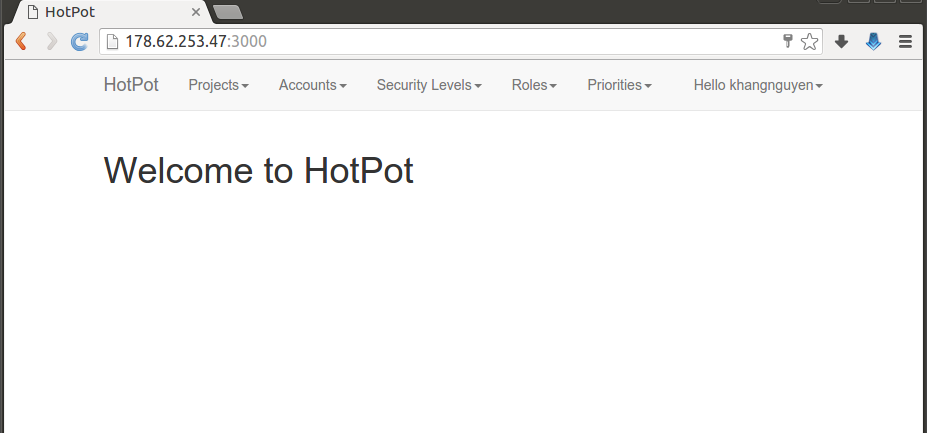
\includegraphics[width=1.0\linewidth]{gfx/chapter_5/general/admin_interface}
\caption[HotPot admin interface]{HotPot admin interface}
\label{fig:user_guide:admin_interface}
\end{figure}

\begin{figure}[bth]                                                                                                                                                  \myfloatalign
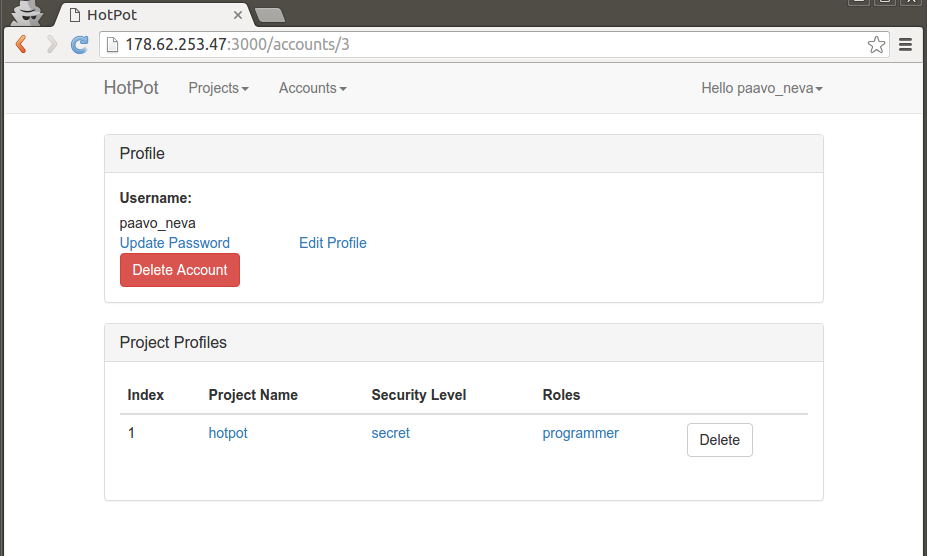
\includegraphics[width=1.0\linewidth]{gfx/chapter_5/general/profile}
\caption[HotPot profile page]{HotPot profile page}
\label{fig:user_guide:profile}
\end{figure}

\begin{figure}[bth]                                                                                                                                                  \myfloatalign
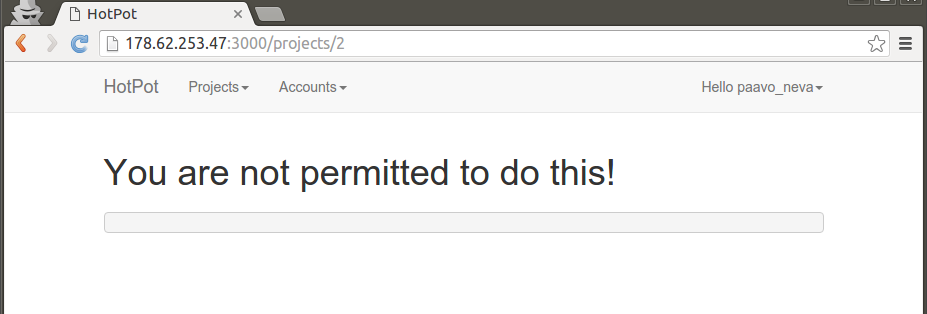
\includegraphics[width=1.0\linewidth]{gfx/chapter_5/general/not_permitted}
\caption[HotPot not permitted error]{HotPot not permitted error}
\label{fig:user_guide:not_permitted}
\end{figure}

\clearpage

\subsubsection{Login}
\label{ch:result:user_guide:miscellaneous:login}

\begin{description}
\item[Description] Every accounts can login to the system using its username and password.
\item[Parameters] An account whose username:password are:
\begin{itemize}
\item \emph{username}: paavo\_neva.
\item \emph{password}: paavo\_neva.
\end{itemize}
\item[Results] If the account is authenticated then a token is created and save on client cookies, and the user is redirected to homepage.
If the account is invalid, the login page will be rendered with error messages.
\end{description}

On homepage \autoref{fig:user_guide:homepage} click on \emph{Log in} link on the top bar to go to \href{http://178.62.253.47:3000/login}{http://178.62.253.47:3000/login}.

\begin{figure}[bth]                                                                                                                                                  \myfloatalign
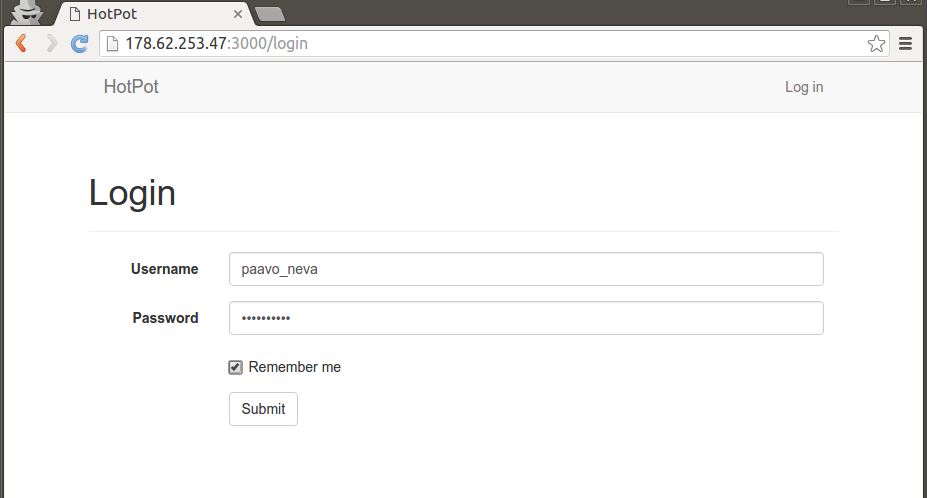
\includegraphics[width=1.0\linewidth]{gfx/chapter_5/miscellaneous/login}
\caption[HotPot login page]{HotPot login page}
\label{fig:user_guide:miscellaneous:login}
\end{figure}

\begin{figure}[bth]
\myfloatalign
\subfloat[Login failed]
{
\label{fig:user_guide:miscellaneous:login_failed}
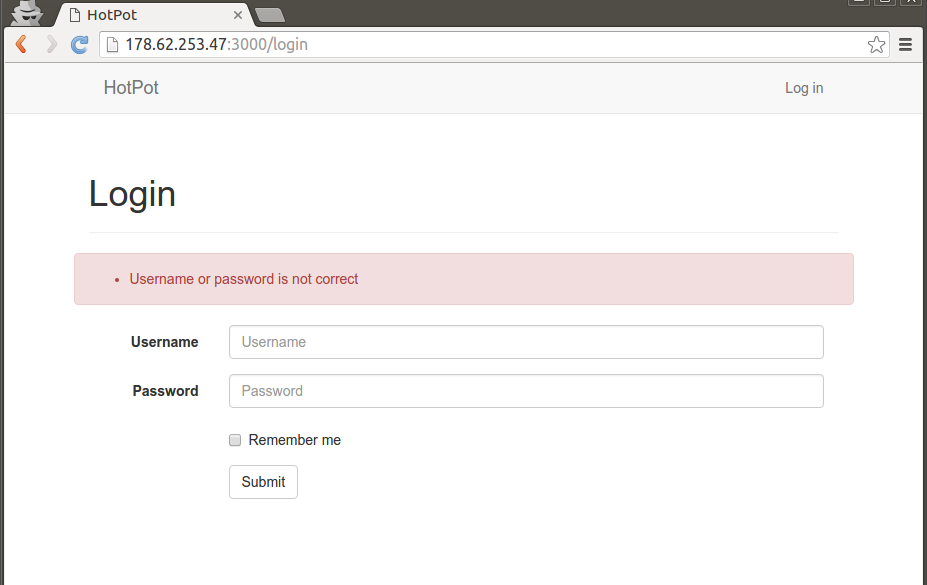
\includegraphics[width=1.\linewidth]{gfx/chapter_5/miscellaneous/login_failed}
} \quad
\subfloat[Login successfully then redirected to profile page]
{
\label{fig:user_guide:miscellaneous:profile}
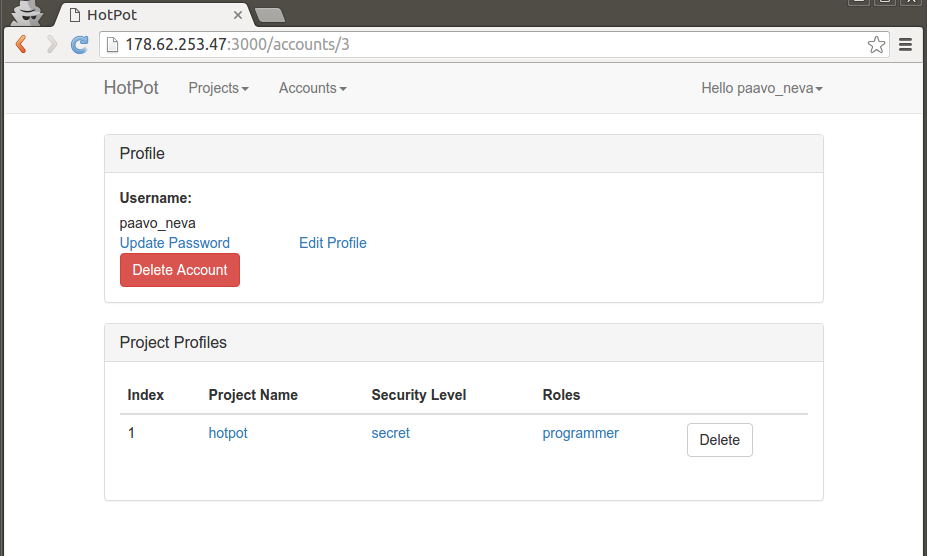
\includegraphics[width=1.\linewidth]{gfx/chapter_5/general/profile}
} \\
\caption[Login results]{Login results}
\label{fig:user_guide:login:result}
\end{figure}

\clearpage

\subsubsection{Logout}
\label{ch:result:user_guide:miscellaneous:logout}

\begin{description}
\item[Description] Every logged in accounts can logout from the system.
\item[Parameters] A logged in account.
\item[Results] The account will be logged out.
Its token will be deleted.
All of his cookies data on the client will be emptied.
Finally, he will be redirected to homepage.
\end{description}

After logging in, on any pages, click on the username link to show \emph{Log out} link.
Click on it for logging out.
After that, the user will be redirected to \emph{homepage} \(\autoref{fig:user_guide:homepage}\).

\begin{figure}[bth]                                                                                                                                                  \myfloatalign
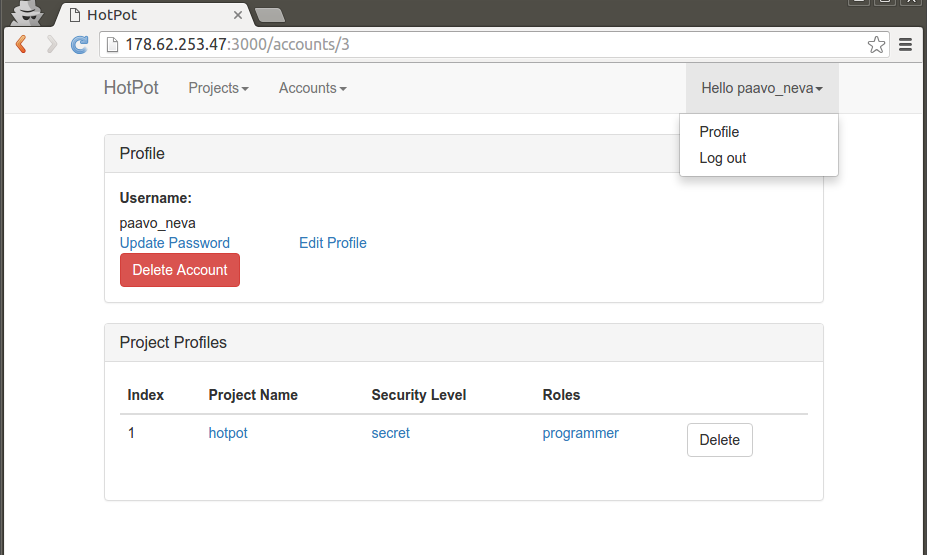
\includegraphics[width=1.0\linewidth]{gfx/chapter_5/miscellaneous/logout}
\caption[HotPot logout link]{HotPot logout link}
\label{fig:user_guide:miscellaneous:logout}
\end{figure}

%\clearpage

% Account guide ----------------------------
\subsection{Account}
\label{ch:result:user_guide:account}
\subsubsection{Create}
\label{ch:result:user_guide:account:create}

\begin{description}
\item[Description] Administrators can create new accounts on the system.
\item[Pre-conditions] An administrator account is logged in.
\item[Parameters] Create an account with values:
\begin{itemize}
\item \emph{username}: testingtesting.
\item \emph{password}: testingtesting.
\end{itemize}
\item[Results] If all the input information is valid, new account will be created, otherwise error messages will be displayed.
\end{description}

After logging in as an administrator, the user interface will appeared like in \autoref{fig:user_guide:admin_interface}.
On the tool bar, click on \emph{Accounts}, then \emph{Create account}.
The creating page will appear under URL

\noindent\href{http://178.62.253.47:3000/accounts/create}{http://178.62.253.47:3000/accounts/create} as shown in \autoref{fig:user_guide:account:account_create}.
Input the value, the \emph{Confirm Password} field is for re-typing password, and the result will be shown as \autoref{fig:user_guide:account:account_create_result}.

\begin{figure}[bth]
\myfloatalign
\subfloat[HotPot Account creation link]
{
\label{fig:user_guide:account:account_create_link}
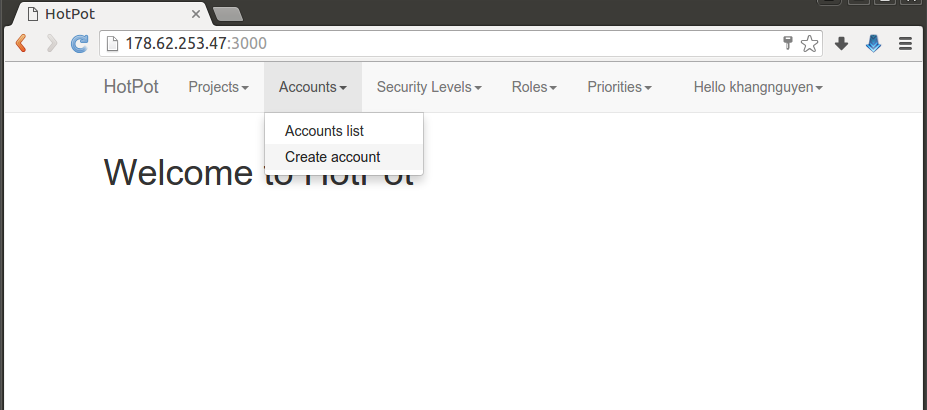
\includegraphics[width=1.0\linewidth]{gfx/chapter_5/account/account_create_link}
} \quad
\subfloat[HotPot Account creating page]
{
\label{fig:user_guide:account:account_create}
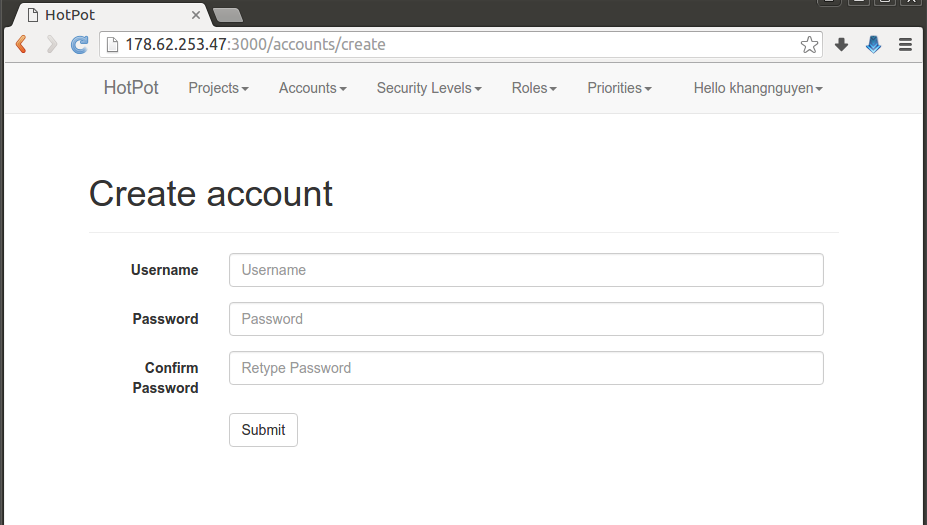
\includegraphics[width=1.0\linewidth]{gfx/chapter_5/account/account_create}
} \\
\caption[HotPot Account creation]{HotPot Account creating}
\label{fig:user_guide:account:account_create}
\end{figure}

\begin{figure}[bth]
\myfloatalign
\subfloat[Account creating failed]
{
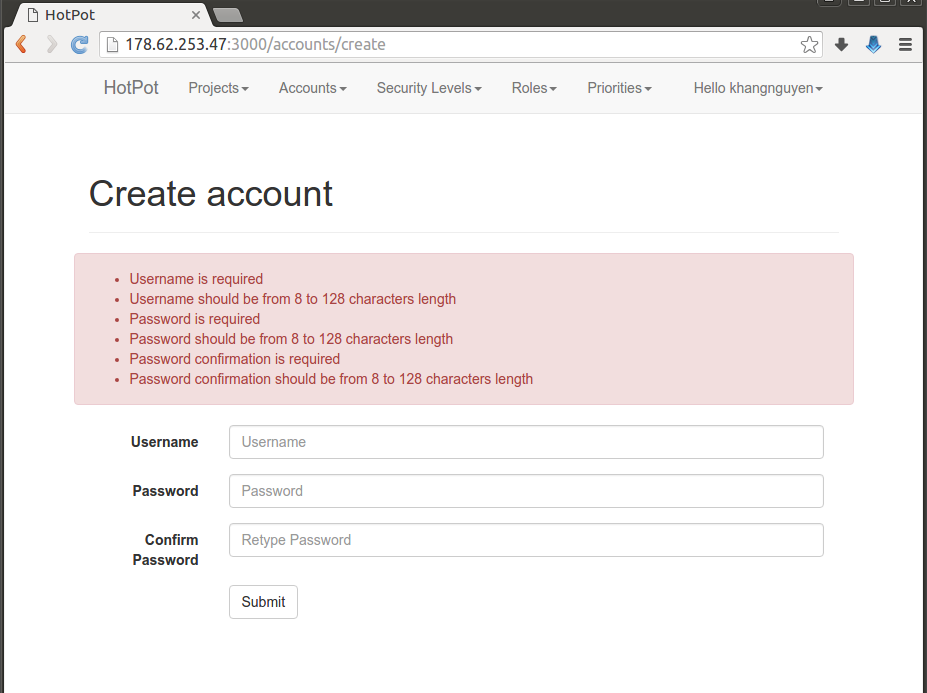
\includegraphics[width=1.\linewidth]{gfx/chapter_5/account/account_create_failed}
} \quad
\subfloat[Account creating successfully then redirected to account detail page]
{
\label{fig:user_guide:account:account_view}
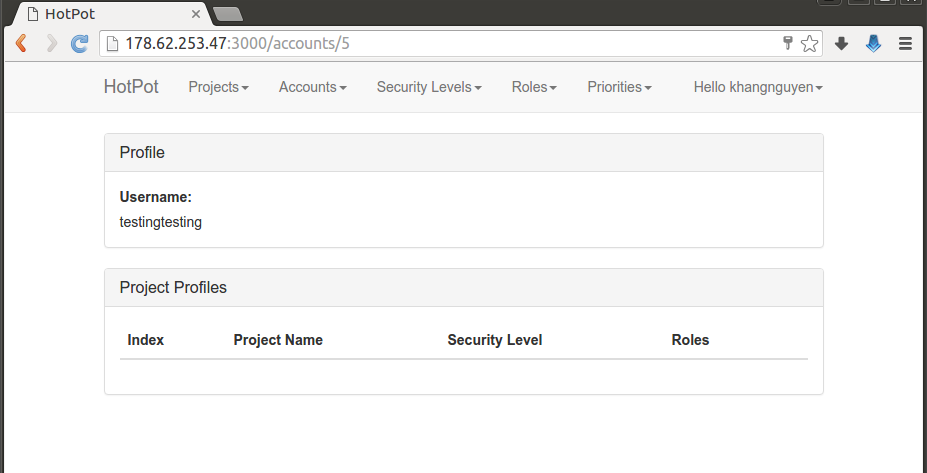
\includegraphics[width=1.\linewidth]{gfx/chapter_5/account/account_view}
} \\
\caption[Login results]{Account creating results}
\label{fig:user_guide:account:account_create_result}
\end{figure}

\clearpage

\subsubsection{Edit profile}
\label{ch:result:user_guide:account:profile}

\begin{description}
\item[Description] Account's owner can edit his all profile details.
\item[Pre-conditions] An account is logged in.
\item[Parameters] Update the logged in account's profile with values:
\begin{itemize}
\item \emph{fullname}: Paavo Neva.
\item \emph{email}: paavo@hotpot.com.
\end{itemize}
\item[Results] If all the input information is valid, the account's profile will be updated.
\end{description}

After logging in, the user interface will appeared like in \autoref{fig:user_guide:user_interface}.
On the tool bar, click on the account name on left top corner, then \emph{Profile} as shown in \autoref{fig:user_guide:account:profile_link}.
The account's profile page will appear under URL \href{http://178.62.253.47:3000/accounts/3}{http://178.62.253.47:3000/accounts/3} as shown in \autoref{fig:user_guide:profile}.
Click on \emph{Edit Profile} link, to go to \href{http://178.62.253.47:3000/accounts/update\_detail}{http://178.62.253.47:3000/accounts/update\_detail} as shown in 
\autoref{fig:user_guide:account:edit_profile}
Input the value, and the result will be shown as \autoref{fig:user_guide:account:profile_updated}.

\begin{figure}[bth]
\myfloatalign
\subfloat[HotPot Profile update link]
{
\label{fig:user_guide:account:profile_link}
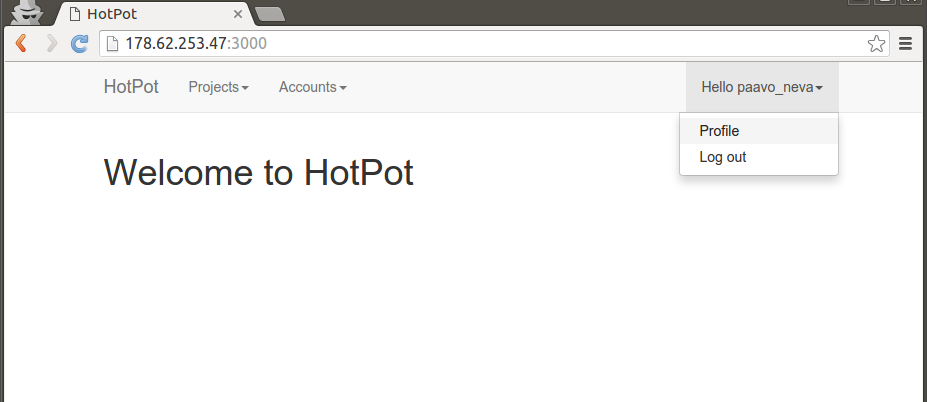
\includegraphics[width=1.0\linewidth]{gfx/chapter_5/account/profile_link}
} \quad
\subfloat[HotPot Profile editing page]
{
\label{fig:user_guide:account:edit_profile}
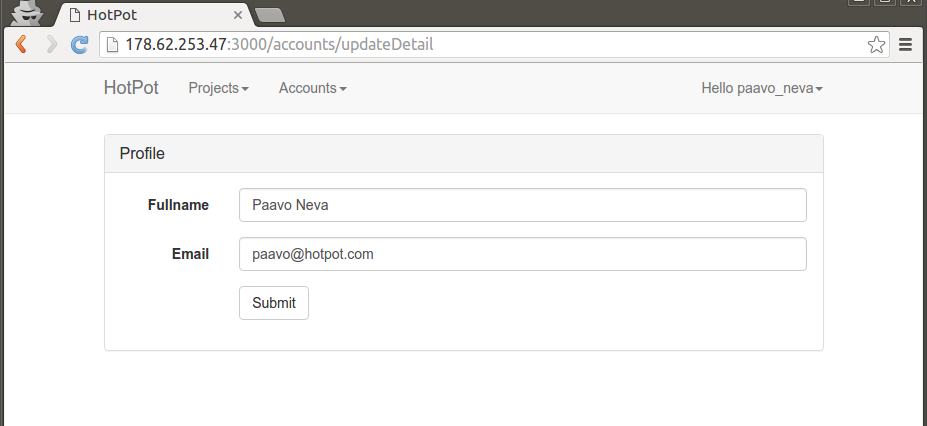
\includegraphics[width=1.0\linewidth]{gfx/chapter_5/account/edit_profile}
} \\
\caption[HotPot Account creation]{HotPot Account creating}
\label{fig:user_guide:account:edit_profile}
\end{figure}

\begin{figure}[bth]                                                                                                                                                  \myfloatalign
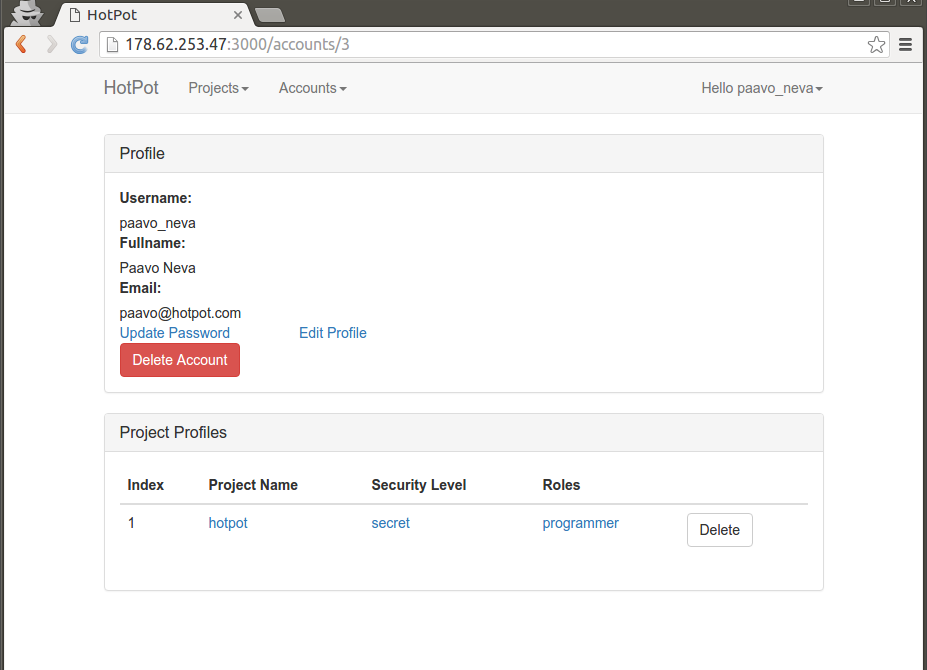
\includegraphics[width=1.0\linewidth]{gfx/chapter_5/account/profile_updated}
\caption[HotPot Profile updated]{HotPot Profile updated}
\label{fig:user_guide:account:profile_updated}
\end{figure}

\subsubsection{Change Password}
\label{ch:result:user_guide:account:change_password}

\begin{description}
\item[Description] Account's owner can change his password.
\item[Pre-conditions] An account is logged in.
\item[Parameters] Update the logged in account's password with values:
\begin{itemize}
\item \emph{password}: newpasswordupdate.
\end{itemize}
\item[Results] If the new password is valid, the user will be redirected back to his profile page.
\end{description}

On user's profile page \(\autoref{fig:user_guide:profile}\), click \emph{Update Password} to go to \href{http://178.62.253.47:3000/accounts/update\_password}{http://178.62.253.47:3000/accounts/update\_password}.
Input new password.
If the new password is valid, the user will be redirected to \autoref{fig:user_guide:profile}, otherwise error messages will be shown as \autoref{fig:user_guide:account:change_password_failed}.

\begin{figure}[bth]                                                                                                                                                  \myfloatalign
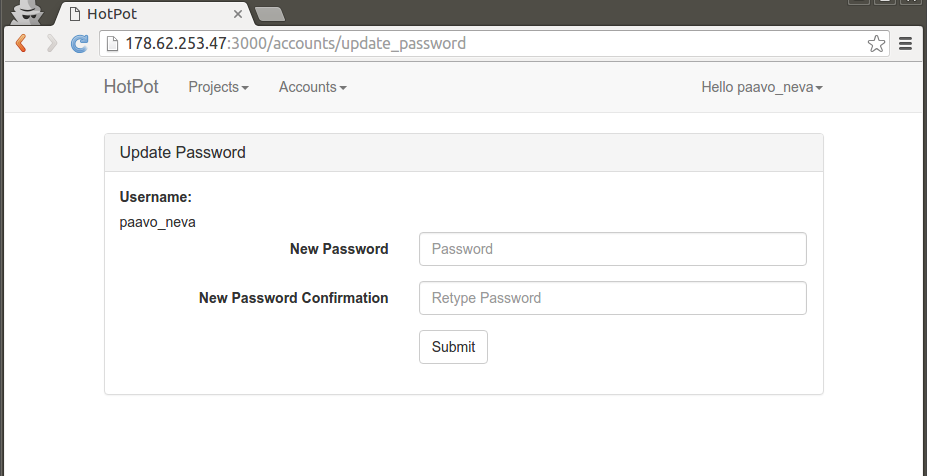
\includegraphics[width=1.0\linewidth]{gfx/chapter_5/account/change_password}
\caption[HotPot password changing page]{HotPot password changing page}
\label{fig:user_guide:account:change_password}
\end{figure}

\begin{figure}[bth]                                                                                                                                                  \myfloatalign
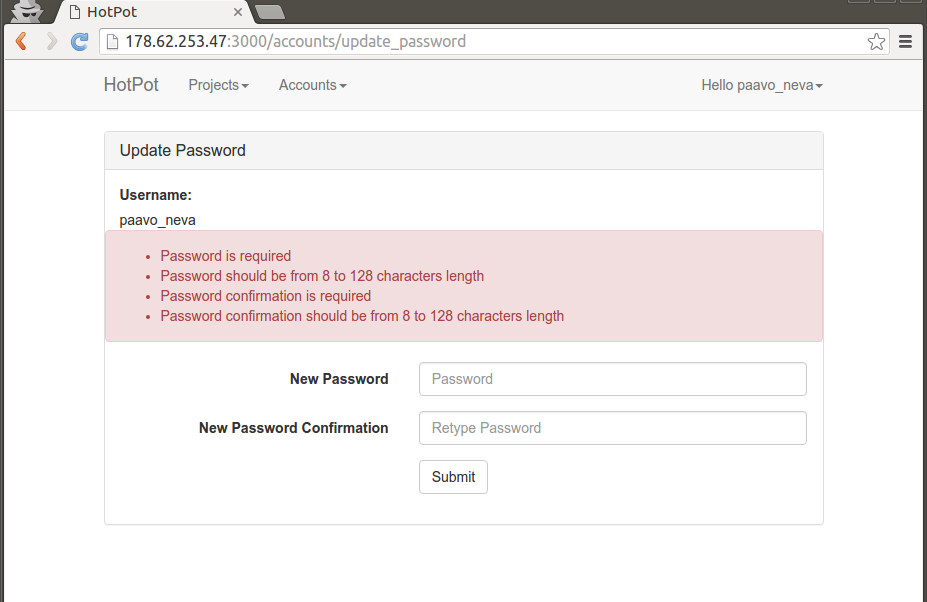
\includegraphics[width=1.0\linewidth]{gfx/chapter_5/account/change_password_failed}
\caption[Password changing failed]{Password changing failed}
\label{fig:user_guide:account:change_password_failed}
\end{figure}

\clearpage

\subsubsection{Delete}
\label{ch:result:user_guide:account:delete}

\begin{description}
\item[Description] Account's owner can delete his account.
\item[Pre-conditions] An account is logged in.
\item[Results] The account will be deleted from the system.
\end{description}

On profile page \autoref{fig:user_guide:profile}, click on \emph{Delete Account} button.

\subsubsection{List and View}
\label{ch:result:user_guide:account:list}

\begin{description}
\item[Description] Every accounts can view the accounts list and their profile.
\item[Pre-conditions] An account is logged in.
\end{description}

On any pages, click on \emph{Accounts} link on top bar, then click on \emph{Account list} link to go to \href{http://178.62.253.47:3000/accounts}{http://178.62.253.47:3000/accounts} as shown in \autoref{fig:user_guide:account:account_list}.
Then, clicking on any user's name to go to account view, as shown in \autoref{fig:user_guide:account:account_view}.

\begin{figure}[bth]
\myfloatalign
\subfloat[HotPot Account list link]
{
\label{fig:user_guide:account:list_link}
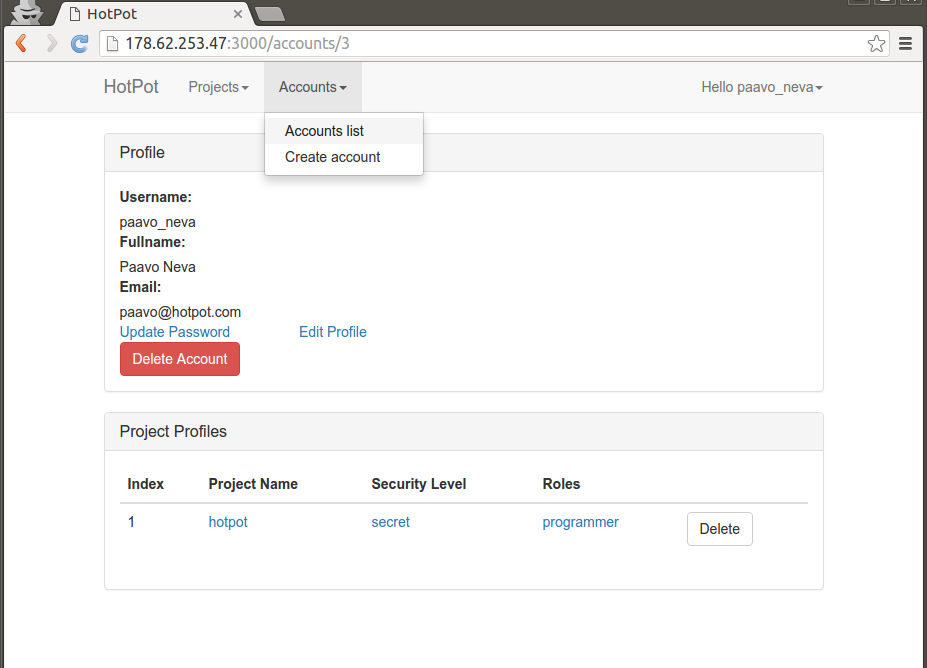
\includegraphics[width=1.0\linewidth]{gfx/chapter_5/account/account_list_link}
} \quad
\subfloat[HotPot Account list page]
{
\label{fig:user_guide:account:account_list}
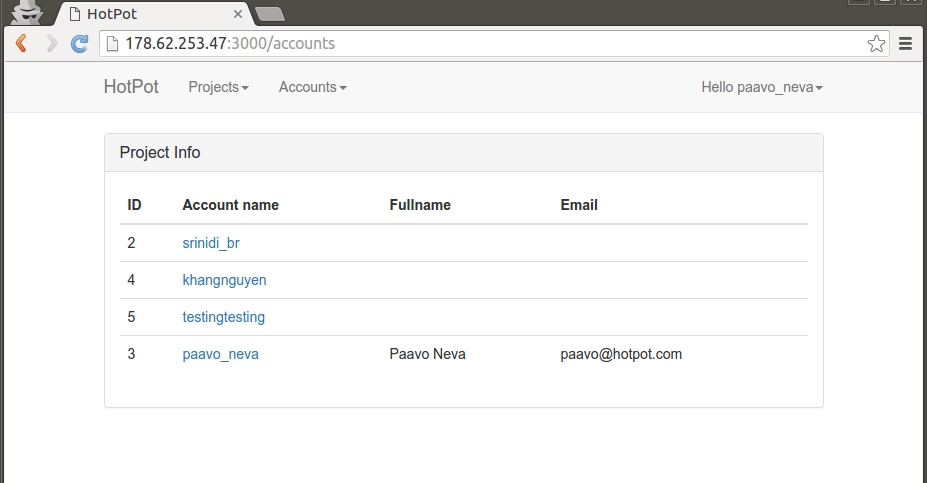
\includegraphics[width=1.0\linewidth]{gfx/chapter_5/account/account_list}
} \\
\caption[HotPot Account list]{HotPot Account list}
\label{fig:user_guide:account:account_list}
\end{figure}

\clearpage

% Project guide ----------------------------
\subsection{Project}
\label{ch:result:user_guide:project}
\subsubsection{Create}
\label{ch:result:user_guide:project:create}

\begin{description}
\item[Description] Every account can create a new project.
\item[Pre-conditions] A logged in account.
\item[Parameters] Create an project with values:
\begin{itemize}
\item \emph{name}: Paavo Project.
\item \emph{description}:  This project is created by paavo\_neva.
\item \emph{due date}: 02/29/2016.
\end{itemize}
\item[Results] If all the input information is valid, new project will be created, the account will be marked as its owner, and the owner will be its first member.
\end{description}

After logging in, on the tool bar, click on \emph{Projects}, then \emph{Create project} as shown in as shown in \autoref{fig:user_guide:project:project_create_link}.
The creating page will appear under URL \href{http://178.62.253.47:3000/projects/create}{http://178.62.253.47:3000/projects/create} as shown in \autoref{fig:user_guide:project:project_create}.
Input the value and the result will be shown as \autoref{fig:user_guide:project:project_create_result}.

\begin{figure}[bth]
\myfloatalign
\subfloat[HotPot Project creation link]
{
\label{fig:user_guide:project:project_create_link}
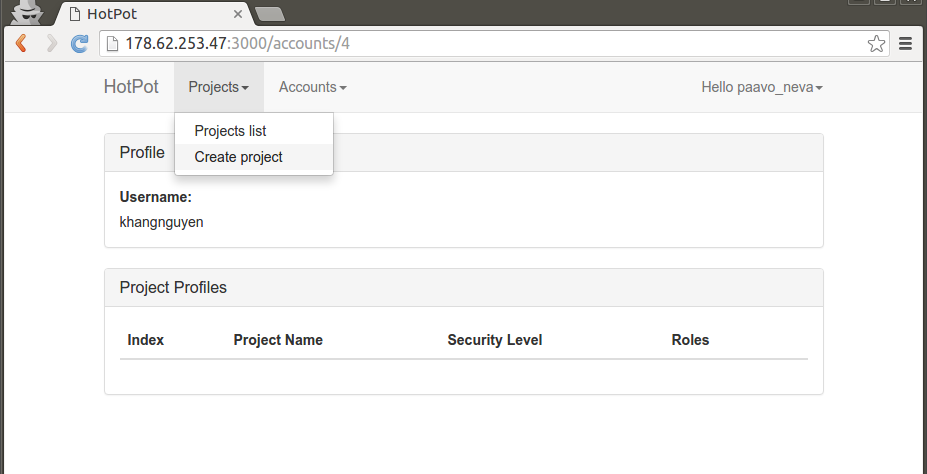
\includegraphics[width=1.0\linewidth]{gfx/chapter_5/project/project_create_link}
} \quad
\subfloat[HotPot Project creating page]
{
\label{fig:user_guide:project:project_create}
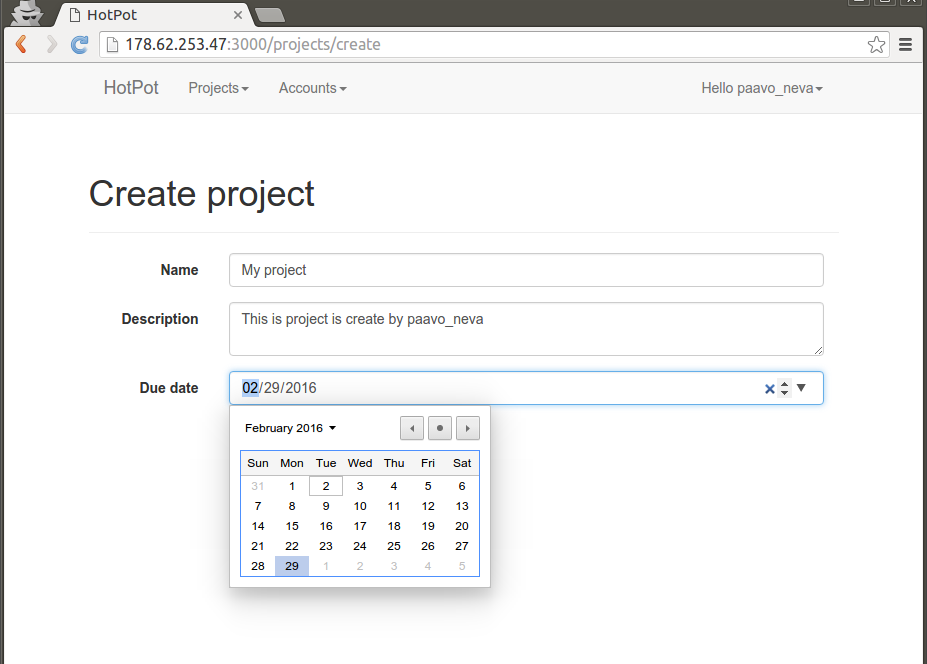
\includegraphics[width=1.0\linewidth]{gfx/chapter_5/project/project_create}
} \\
\caption[HotPot Project creation]{HotPot Project creating}
\label{fig:user_guide:project:project_create}
\end{figure}

\begin{figure}[bth]
\myfloatalign
\subfloat[Project creating failed]
{
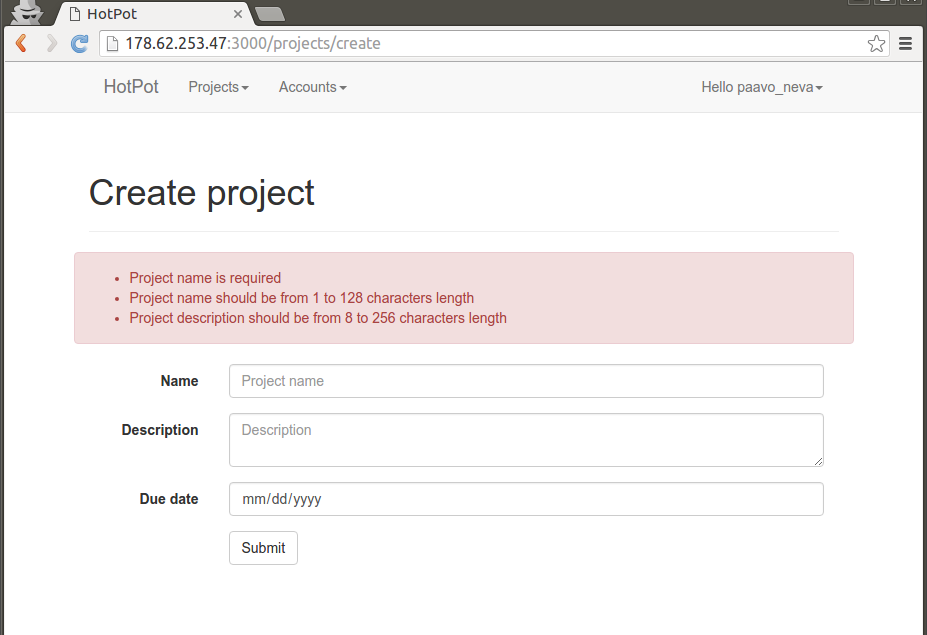
\includegraphics[width=1.\linewidth]{gfx/chapter_5/project/project_create_failed}
} \quad
\subfloat[Project creating successfully then redirected to project detail page]
{
\label{fig:user_guide:project:project_view}
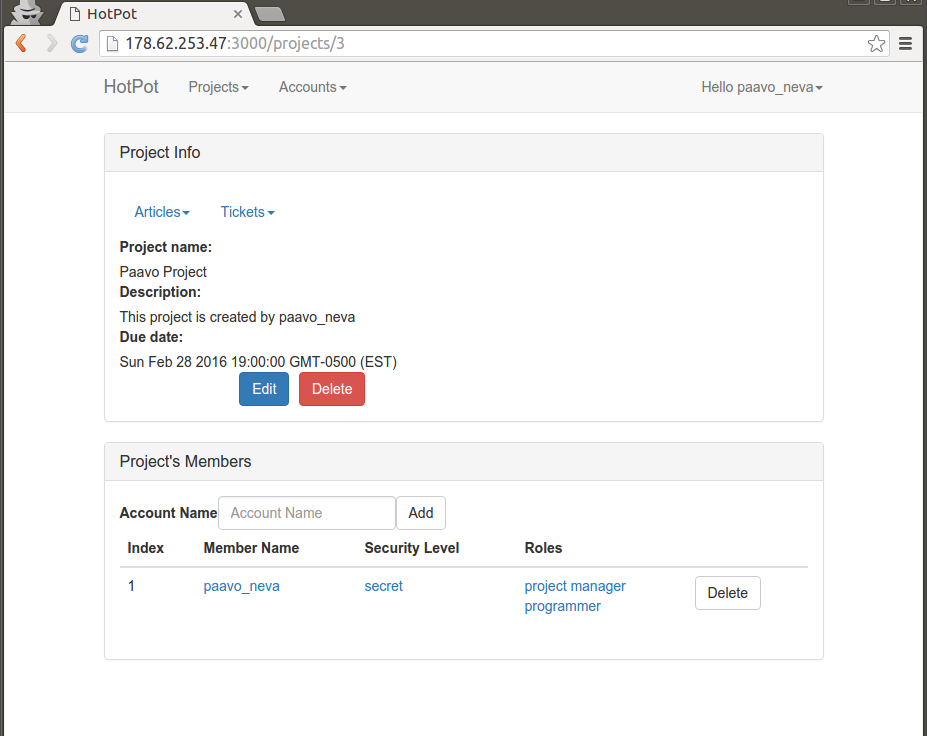
\includegraphics[width=1.\linewidth]{gfx/chapter_5/project/project_view}
} \\
\caption[Project creating results]{Project creating results}
\label{fig:user_guide:project:project_create_result}
\end{figure}

\clearpage

\subsubsection{Managing member}
\label{ch:result:user_guide:project:managing_member}

\begin{description}
\item[Description] Only project owner can add or remove project's member.
\item[Pre-conditions] Project's owner logged in, \eg account \emph{paavo\_neva}.
\item[Parameters] Add and remove user \emph{srinidi\_br} to/from \emph{Paavo Project} project.
\item[Results] The account will respectively be added and removed from \emph{Paavo Project} project.
\end{description}

After logging in as the project's owner, go to his own project in URL \href{http://178.62.253.47:3000/projects/3}{http://178.62.253.47:3000/projects/3}.
Input the \emph{account's name} and the result will be shown as \autoref{fig:user_guide:project:assign_member}.

For removing project's member, on the project view, click on the member's \emph{Delete} button.

\begin{figure}[bth]
\myfloatalign
\subfloat[Project: inputting project's new member username]
{
\label{fig:user_guide:project:input_new_member}
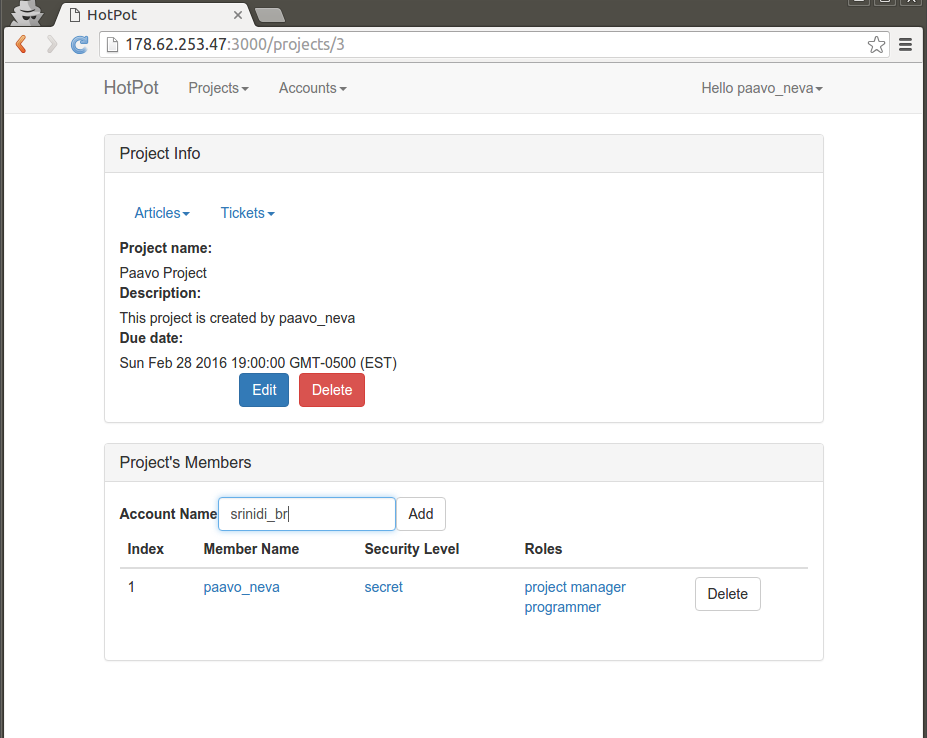
\includegraphics[width=1.\linewidth]{gfx/chapter_5/project/assign_member}
} \quad
\subfloat[Project: assigning project's new member successfully]
{
\label{fig:user_guide:project:project_view}
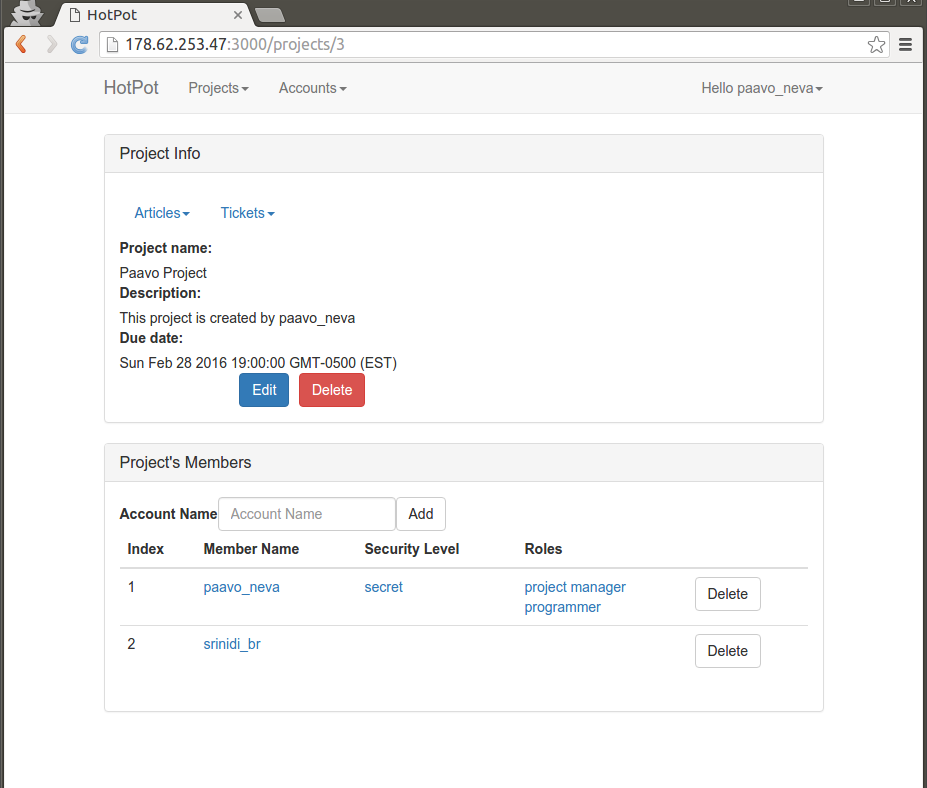
\includegraphics[width=1.\linewidth]{gfx/chapter_5/project/assign_member_successfully}
} \\
\caption[Project: assigning project's new member]{Project: assigning project's new member}
\label{fig:user_guide:project:assign_member}
\end{figure}

\clearpage

\subsubsection{Update}
\label{ch:result:user_guide:project:update}

\begin{description}
\item[Description] Only project owner can edit his own project.
\item[Pre-conditions] Project's owner logged in, \eg account \emph{paavo\_neva}.
\item[Results] The project will be updated with new details.
\end{description}

After logging in as the project's owner, on the project view page, as shown in \autoref{fig:user_guide:project:project_view}, click \emph{Edit} button to go to its edit page 

\noindent\href{http://178.62.253.47:3000/projects/edit/3}{http://178.62.253.47:3000/projects/edit/3}.
Change the project's details.
If there are any errors, they will be shown as \autoref{fig:user_guide:project:project_edit_failed}, otherwise the user will be redirected to project view.

\begin{figure}[bth]
\myfloatalign
\subfloat[Project: edit page]
{
\label{fig:user_guide:project:project_edit_page}
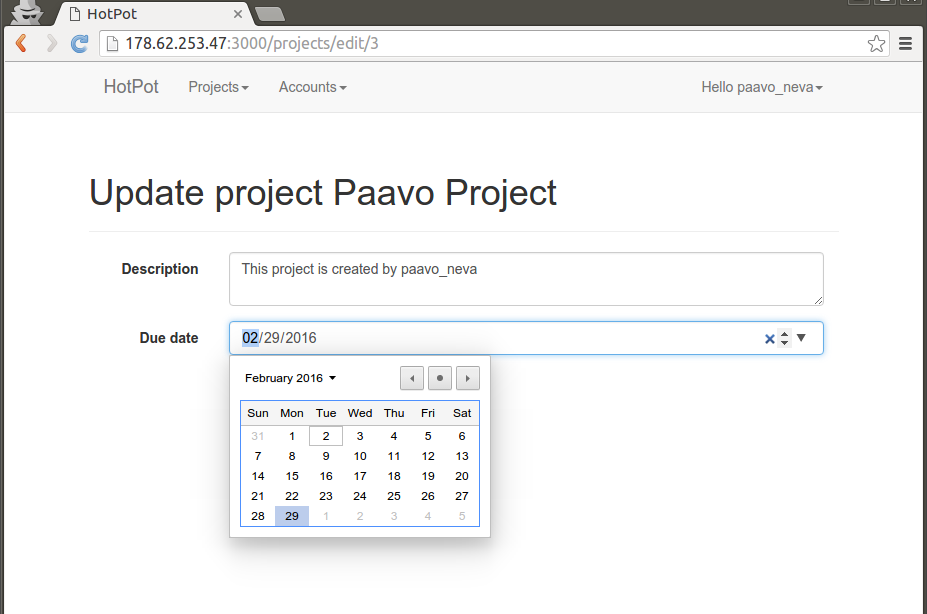
\includegraphics[width=1.\linewidth]{gfx/chapter_5/project/project_edit}
} \quad
\subfloat[Project: project editing failed]
{
\label{fig:user_guide:project:project_edit_failed}
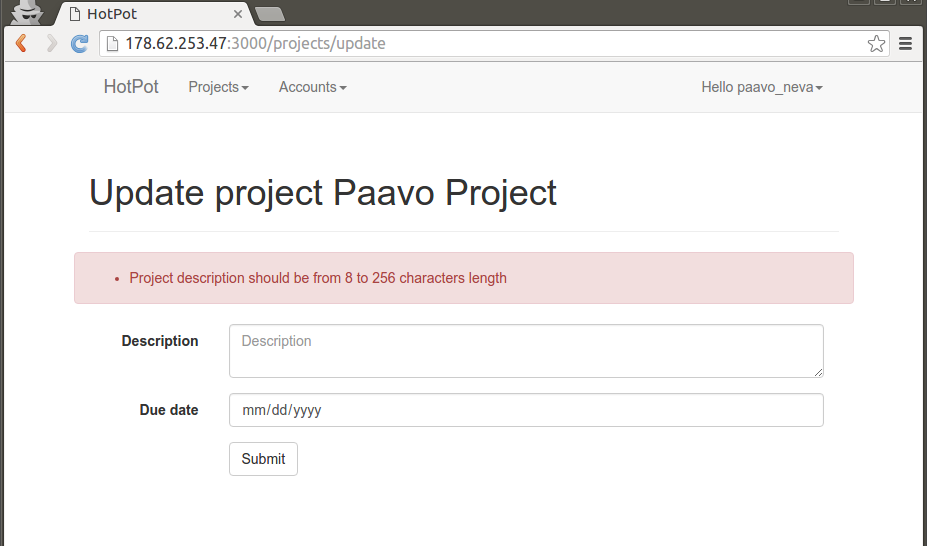
\includegraphics[width=1.\linewidth]{gfx/chapter_5/project/project_edit_failed}
} \\
\caption[Project: project edit]{Project:  project edit}
\label{fig:user_guide:project:project_edit}
\end{figure}

\clearpage

\subsubsection{Delete}
\label{ch:result:user_guide:project:delete}

\begin{description}
\item[Description] Only project owner can delete his own project.
\item[Pre-conditions] Project's owner logged in, \eg account \emph{paavo\_neva}.
\item[Results] The project will be deleted.
\end{description}

After logging in as the project's owner, on the project view page, as shown in \autoref{fig:user_guide:project:project_view}, click \emph{Delete} button to delete the current project. 

\subsubsection{List and View}
\label{ch:result:user_guide:project:list}

\begin{description}
\item[Description] Every accounts can view the list of projects. However, only the team member can view the project's details.
\item[Pre-conditions] A logged in account, \eg account \emph{paavo\_neva}.
\item[Results] The user can view the list of all projects, but can only see details of projects in which he is a team member.
\end{description}

After logging in, in every pages, on the top bar, click on \emph{Projects} link, then click on \emph{Projects list}, as shown in \autoref{fig:user_guide:project:project_list_link}, to go to 

\noindent\href{http://178.62.253.47:3000/projects}{http://178.62.253.47:3000/projects} as shown in \autoref{fig:user_guide:project:project_list}.
Then clicking on any project's name will go to the project's view page, as \autoref{fig:user_guide:project:project_view}, if the user is a member of the project, otherwise \autoref{fig:user_guide:not_permitted} will be shown.

\begin{figure}[bth]
\myfloatalign
\subfloat[Project: projects list link]
{
\label{fig:user_guide:project:project_list_link}
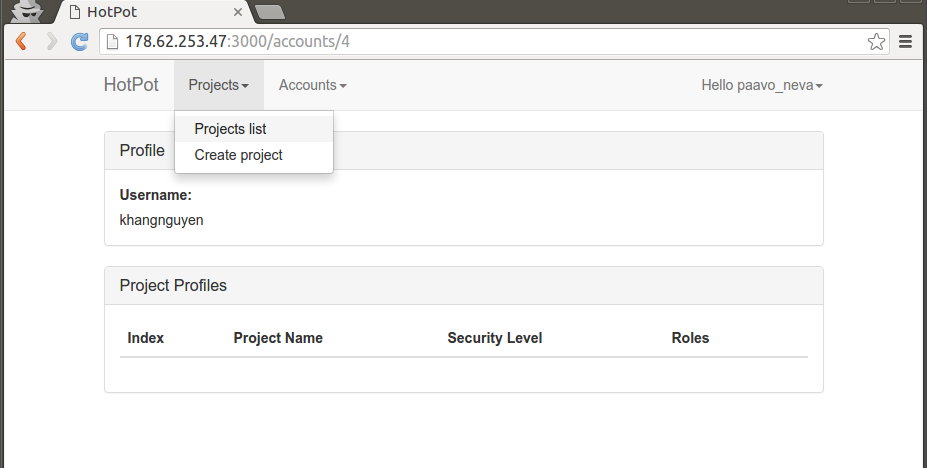
\includegraphics[width=1.\linewidth]{gfx/chapter_5/project/project_list_link}
} \quad
\subfloat[Project: projects list]
{
\label{fig:user_guide:project:project_list}
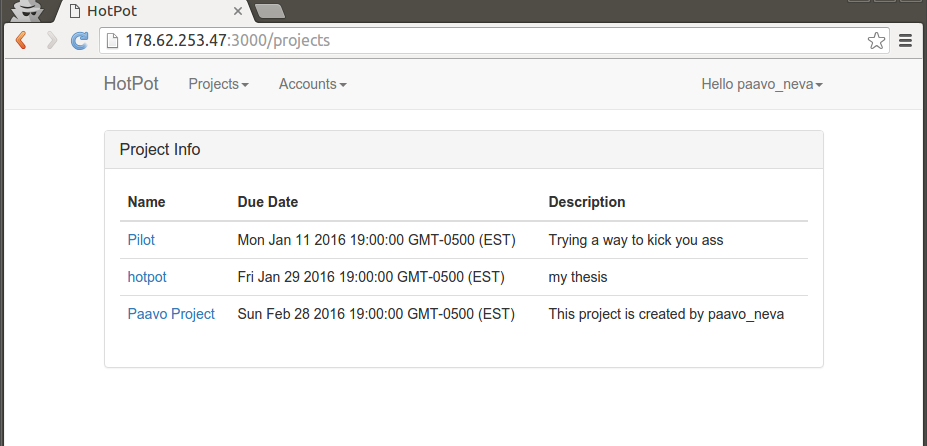
\includegraphics[width=1.\linewidth]{gfx/chapter_5/project/project_list}
} \\
\caption[Project: view projects list]{Project: view projects list}
\label{fig:user_guide:project:project_list}
\end{figure}

\clearpage

% Article guide ----------------------------
\subsection{Article}
\label{ch:result:user_guide:article}
\subsubsection{Create}
\label{ch:result:user_guide:article:create}

\begin{description}
\item[Description] Only project members can create the project's new articles.
\item[Pre-conditions] Project's member logged in, \eg account \emph{paavo\_neva} and project \emph{Paavo Project}.
\item[Conditions] The article's \emph{security level} can only be equal or higher than its creator's.
\item[Parameters] Create new article with these values:
\begin{itemize}
\item \emph{name}: Paavo article.
\item \emph{description}: This article is created by Paavo.
\item \emph{content}: A secret content.
\item \emph{is directory}: false.
\item \emph{writable}: true.
\item \emph{readable}: true.
\item \emph{security level}: secret (equals to account \emph{paavo\_neva}).
\item \emph{role}: designer and programmer.
\end{itemize}
\item[Results] A new artilce will be created under the project.
\end{description}

\subsubsection{Update}
\label{ch:result:user_guide:article:update}

\begin{description}
\item[Description] Only project members can update the project's articles.
Furthemore, the member must either be the article's owner or have a set of security policies which satisfies the article's one.
The access control logics were discussed in \autoref{ch:hopot_project:project_components}.
\item[Pre-conditions] Project's member logged in, an article is created as \autoref{ch:result:user_guide:article:create}.
\item[Conditions] The article's new \emph{security level} can only be equal or higher than its creator's.
\item[Parameters] Update the article with these values:
\begin{itemize}
\item \emph{name}: Paavo article.
\item \emph{description}: This updated article is created by Paavo.
\item \emph{content}: A top secret content.
\item \emph{is directory}: false.
\item \emph{writable}: true.
\item \emph{readable}: true.
\item \emph{security level}: top secret (equals to account \emph{paavo\_neva}).
\item \emph{role}: programmer.
\end{itemize}
\item[Results] If the input values are valid, the artilce will be updated accordingly.
\end{description}

\subsubsection{Delete}
\label{ch:result:user_guide:article:delete}

\begin{description}
\item[Description] Only article's owner can delete it.
\item[Pre-conditions] An article is created as \autoref{ch:result:user_guide:article:create}.
The article's owner logged in.
\item[Results] The article will be deleted.
\end{description}

\subsubsection{List}
\label{ch:result:user_guide:article:list}

\begin{description}
\item[Description] Only project's members can see the list of articles in that project.
Articles in the list are filtered upon the member's set of security labels, as discussed in \autoref{ch:hopot_project:project_components}.
\item[Pre-conditions] Project's member logged in.
\item[Results] List of filtered articles.
\end{description}

\subsubsection{View}
\label{ch:result:user_guide:article:list}

\begin{description}
\item[Description] Only project's members can view article's details in that project.
Furthemore, the member must either be the article's owner or have a set of security policies which satisfies the article's one.
The access control logics were discussed in \autoref{ch:hopot_project:project_components}.
\item[Pre-conditions] Project's member logged in.
\item[Results] View the article's details.
\end{description}

% Ticket guide ----------------------------
\subsection{Ticket}
\label{ch:result:user_guide:ticket}
\subsubsection{Create}
\label{ch:result:user_guide:ticket:create}

\begin{description}
\item[Description] Only project members can create the project's new tickets.
\item[Pre-conditions] Project's member logged in, \eg account \emph{paavo\_neva} and project \emph{Paavo Project}.
\item[Conditions] The ticket's \emph{security level} can only be equal or higher than its creator's.
\item[Parameters] Create new ticket with these values:
\begin{itemize}
\item \emph{name}: Paavo ticket.
\item \emph{content}: A secret content.
\item \emph{due date}: 02/29/2016.
\item \emph{writable}: true.
\item \emph{readable}: true.
\item \emph{priority}: normal.
\item \emph{security level}: secret (equals to account \emph{paavo\_neva}).
\item \emph{role}: designer and programmer.
\end{itemize}
\item[Results] A new artilce will be created under the project.
\end{description}

\subsubsection{Update}
\label{ch:result:user_guide:ticket:update}

\begin{description}
\item[Description] Only project members can update the project's tickets.
Furthemore, the member must either be the ticket's owner or have a set of security policies which satisfies the ticket's one.
The access control logics were discussed in \autoref{ch:hopot_project:project_components}.
\item[Pre-conditions] Project's member logged in, an ticket is created as \autoref{ch:result:user_guide:ticket:create}.
\item[Conditions] The ticket's new \emph{security level} can only be equal or higher than its creator's.
\item[Parameters] Update the ticket with these values:
\begin{itemize}
\item \emph{name}: Paavo ticket.
\item \emph{content}: A top secret content.
\item \emph{due date}: 02/29/2016.
\item \emph{writable}: true.
\item \emph{readable}: true.
\item \emph{priority}: high.
\item \emph{security level}: top secret (equals to account \emph{paavo\_neva}).
\item \emph{role}: programmer.
\end{itemize}
\item[Results] If the input values are valid, the artilce will be updated accordingly.
\end{description}

\subsubsection{Delete}
\label{ch:result:user_guide:ticket:delete}

\begin{description}
\item[Description] Only ticket's owner can delete it.
\item[Pre-conditions] An ticket is created as \autoref{ch:result:user_guide:ticket:create}.
The ticket's owner logged in.
\item[Results] The ticket will be deleted.
\end{description}

\subsubsection{List}
\label{ch:result:user_guide:ticket:list}

\begin{description}
\item[Description] Only project's members can see the list of tickets in that project.
tickets in the list are filtered upon the member's set of security labels, as discussed in \autoref{ch:hopot_project:project_components}.
\item[Pre-conditions] Project's member logged in.
\item[Results] List of filtered tickets.
\end{description}

\subsubsection{View}
\label{ch:result:user_guide:ticket:list}

\begin{description}
\item[Description] Only project's members can view ticket's details in that project.
Furthemore, the member must either be the ticket's owner or have a set of security policies which satisfies the ticket's one.
The access control logics were discussed in \autoref{ch:hopot_project:project_components}.
\item[Pre-conditions] Project's member logged in.
\item[Results] View the ticket's details.
\end{description}

% Security Level guide ----------------------------
\subsection{Security Level}
\label{ch:result:user_guide:security_level}
\subsubsection{Create}
\label{ch:result:user_guide:security_level:create}

\begin{description}
\item[Description] Only administrators can create the system's new security level.
\item[Pre-conditions] A logged in administrator account, \eg account \emph{khangnguyen:khangnguyen}.
\item[Parameters] Create new security level with these values:
\begin{itemize}
\item \emph{name}: God file.
\item \emph{level}: 5 (the higher level the more secured the label is).
\item \emph{description}: Ultimately secret level.
\end{itemize}
\item[Results] A new security level label will be created in the system.
\end{description}

\subsubsection{Update}
\label{ch:result:user_guide:security_level:update}

\begin{description}
\item[Description] Only administrators can update the system's existing security levels.
\item[Pre-conditions] A logged in administrator account, \eg account \emph{khangnguyen:khangnguyen}.
A security level is created as \autoref{ch:result:user_guide:security_level:create}
\item[Parameters] Update the security level with these values:
\begin{itemize}
\item \emph{name}: Sheep file.
\item \emph{level}: 1.
\item \emph{description}: Ultimately low level.
\end{itemize}
\item[Results] The level will be updated.
\end{description}

\subsubsection{Delete}
\label{ch:result:user_guide:security_level:delete}

\begin{description}
\item[Description] Only administrators can delete the system's existing security levels.
\item[Pre-conditions] A logged in administrator account, \eg account \emph{khangnguyen:khangnguyen}.
A security level is created as \autoref{ch:result:user_guide:security_level:create}
\item[Results] The level will be deleted.
\end{description}

\subsubsection{List and View}
\label{ch:result:user_guide:security_level:list}

\begin{description}
\item[Description] Every accounts can view the list of security levels in the system, as well as their details.
\item[Pre-conditions] A logged in account, \eg account \emph{khangnguyen:khangnguyen}.
\item[Results] The list of security levels is shown.
\end{description}

% Role guide ----------------------------
\subsection{Role}
\label{ch:result:user_guide:role}
\subsubsection{Create}
\label{ch:result:user_guide:role:create}

\begin{description}
\item[Description] Only administrators can create the system's new role.
\item[Pre-conditions] A logged in administrator account, \eg account \emph{khangnguyen:khangnguyen}.
\item[Parameters] Create new role with these values:
\begin{itemize}
\item \emph{name}: System admin.
\item \emph{description}: He fix your machine.
\end{itemize}
\item[Results] A new role label will be created in the system.
\end{description}

\subsubsection{Update}
\label{ch:result:user_guide:role:update}

\begin{description}
\item[Description] Only administrators can update the system's existing roles.
\item[Pre-conditions] A logged in administrator account, \eg account \emph{khangnguyen:khangnguyen}.
A role is created as \autoref{ch:result:user_guide:role:create}
\item[Parameters] Update the role with these values:
\begin{itemize}
\item \emph{name}: System admin.
\item \emph{description}: He fix your machine, and back you up.
\end{itemize}
\item[Results] The role will be updated.
\end{description}

\subsubsection{Delete}
\label{ch:result:user_guide:role:delete}

\begin{description}
\item[Description] Only administrators can delete the system's existing roles.
\item[Pre-conditions] A logged in administrator account, \eg account \emph{khangnguyen:khangnguyen}.
A role is created as \autoref{ch:result:user_guide:role:create}
\item[Results] The role will be deleted.
\end{description}

\subsubsection{List and View}
\label{ch:result:user_guide:role:list}

\begin{description}
\item[Description] Every accounts can view the list of roles in the system, as well as their details.
\item[Pre-conditions] A logged in account, \eg account \emph{khangnguyen:khangnguyen}.
\item[Results] The list of roles is shown.
\end{description}

% Priority guide ----------------------------
\subsection{Priority}
\label{ch:result:user_guide:priority}
\subsubsection{Create}
\label{ch:result:user_guide:priority:create}

\begin{description}
\item[Description] Only administrators can create the system's new priority.
\item[Pre-conditions] A logged in administrator account, \eg account \emph{khangnguyen:khangnguyen}.
\item[Parameters] Create new priority with these values:
\begin{itemize}
\item \emph{name}: Highest Priority.
\item \emph{level}: 5 (the higher level the higher the priority is).
\item \emph{description}: Ultimately high priority.
\end{itemize}
\item[Results] A new priority label will be created in the system.
\end{description}

\subsubsection{Update}
\label{ch:result:user_guide:priority:update}

\begin{description}
\item[Description] Only administrators can update the system's existing priorities.
\item[Pre-conditions] A logged in administrator account, \eg account \emph{khangnguyen:khangnguyen}.
A priority is created as \autoref{ch:result:user_guide:priority:create}
\item[Parameters] Update the priority with these values:
\begin{itemize}
\item \emph{name}: Sheep file.
\item \emph{level}: 1.
\item \emph{description}: Ultimately low priority.
\end{itemize}
\item[Results] The priority will be updated.
\end{description}

\subsubsection{Delete}
\label{ch:result:user_guide:priority:delete}

\begin{description}
\item[Description] Only administrators can delete the system's existing priorities.
\item[Pre-conditions] A logged in administrator account, \eg account \emph{khangnguyen:khangnguyen}.
A priority is created as \autoref{ch:result:user_guide:priority:create}
\item[Results] The priority will be deleted.
\end{description}

\subsubsection{List and View}
\label{ch:result:user_guide:priority:list}

\begin{description}
\item[Description] Every accounts can view the list of priorities in the system, as well as their details.
\item[Pre-conditions] A logged in account, \eg account \emph{khangnguyen:khangnguyen}.
\item[Results] The list of priorities is shown.
\end{description}

%----------------------------------------------------------------------------------------
\section{Learnings}

As working on the project, I have learned many new things.
First of all, technically, this is my second \emph{Nodejs} project.
So in this project, I deliberately chose it for study purpose.
After the project, I had an improving about \emph{Nodejs} and one of its most popular framework \emph{Expressjs}.
All of my experiences and learning about it are noted in \emph{diary} directory on GitHub repository which is listed in \autoref{ch:appendix:repository_structure}.
Those diaries are my daily reports of what I have done, the problems occurred on that day, and their solutions if available\dots

About programming experience, there is one advise which may be very useful when we have to due with unfamiliar issues of new technologies: always spend time for reading the technology's documents.
\marginpar{``Give me six hours to chop down a tree and I will spend the first four sharpening the axe'' -- Abraham Lincoln (1809-1865) }
Obviously, with the strong supports of huge technical communities these days, we can easily finish our jobs by searching for available solutions.
However, it doesn't help us to master the technology on our own \ie we don't understand it enough to handle other problems in the future.
Reading documentation will profit us in understand the technology's principles, from that we can study best practices in using it.
Consequently, it will improve our performance in using it.
On the other hand, spending time on learning a technology properly, we will also learn its owner's experience on programming and problems solving skills.
In another word, we can inherit his programming mindsets, design patterns which could be profitable in our future projects.
My suggestion is to put technology studying as a task in the project's tasks list, and assign a time span to it as an usual one.
The time span should be long enough for reading through the technology's documents, and not too long or it will become time consuming.
It took me two days to learn about \emph{Expressjs} enough for me to start working with it initially.
And it takes the same amount of time for me to studying using some crucial libraries such as \emph{Sequelizejs}, \emph{Promise}\dots
And on the working progress, I can learn more about their good practices.

Besides that, studying about MLS is a huge advantage to me.
Security is always a hot and essential topic, MLS is one of it.
Through the project, I learned about the MLS policies, and how they could be implemented in a system.
We have to design a blueprint of the system based on selected MLS model.
The blueprint consists of rules that \emph{subjects} and \emph{objects} of the system must be devoted to.
In the progress, we need to review it multiple times in multiple points of view to ensure that there is no exception.
Rather than that, again, there is no \emph{one master solution for all problems}, sometimes we have to make compromises.
In another word, for example, we have to make trade-off between performance and security.
The high secured system may be complicated and inflexible; however, flexible system with many \emph{trusted subjects/objects} could pose security leaks in the future.
So that, whenever we have to make a compromise, we have to acknowledge and keep in mind (or better, in note) its consequences to avoid in future work.

Planing is also an extensive skill.
Although, this project is my personal project, I learned a lot of time management.
In my own opinion, at the first try, we should assign a task with a small extension of time than we have evaluated.
We should not give a too tight time slot for very first tasks, there will be usually some modifications in features list and project requirements at the first stage of the project; and making early decisions very likely leads to changes.
As the progress goes on, the project is also getting stable.
The number of sudden changes or making decision will decrease remarkably.
Consequently, at this time, we can shorten the addition time extension, or just omit it.

